\section{Metodología}
\subsection{Materiales}
\section*{Estructura del sistema}

\begin{itemize}[leftmargin=1.2cm]
  \item \textbf{Estructura mecánica:}
  \begin{itemize}
    \item MDF de 3.2 a 10 mm (cortado por láser).
    \item Tornillería estándar (M3, tuercas, arandelas, bujes, espaciadores).
  \end{itemize}

  \item \textbf{Actuadores:}
  \begin{itemize}
    \item 4 × Servomotores MG996R de 180° (uno por articulación).
    Según la hoja de datos del MG996R, este servo de engranajes metálicos y doble rodamientos ofrece un par de detención (“stall torque”) de hasta 11 kg·cm a 6 V y una velocidad de 0,14 s por 60° 
components101.com.
  \end{itemize}

  \item \textbf{Efectores:}
  \begin{itemize}
    \item Garra mecánica.
    \item Electroimán para piezas ferromagnéticas.
  \end{itemize}

  \item \textbf{Electrónica de control:}
  \begin{itemize}
    \item Microcontrolador ATmega328P (ejemplo: Arduino Uno/Nano).
    \item Driver MOSFET  para el electroimán.
    \item Finales de carrera (para homing).
    \item LEDs indicadores y buzzer de estado.
  \end{itemize}

  \item \textbf{Fuente de alimentación:}
  \begin{itemize}
    \item Fuente de poder (capaz de alimentar servos y microcontrolador).
    \item Reguladores o convertidores de voltaje según necesidad.
  \end{itemize}
\end{itemize}

\subsection{Software de control}

\begin{figure}[H]
  \centering
  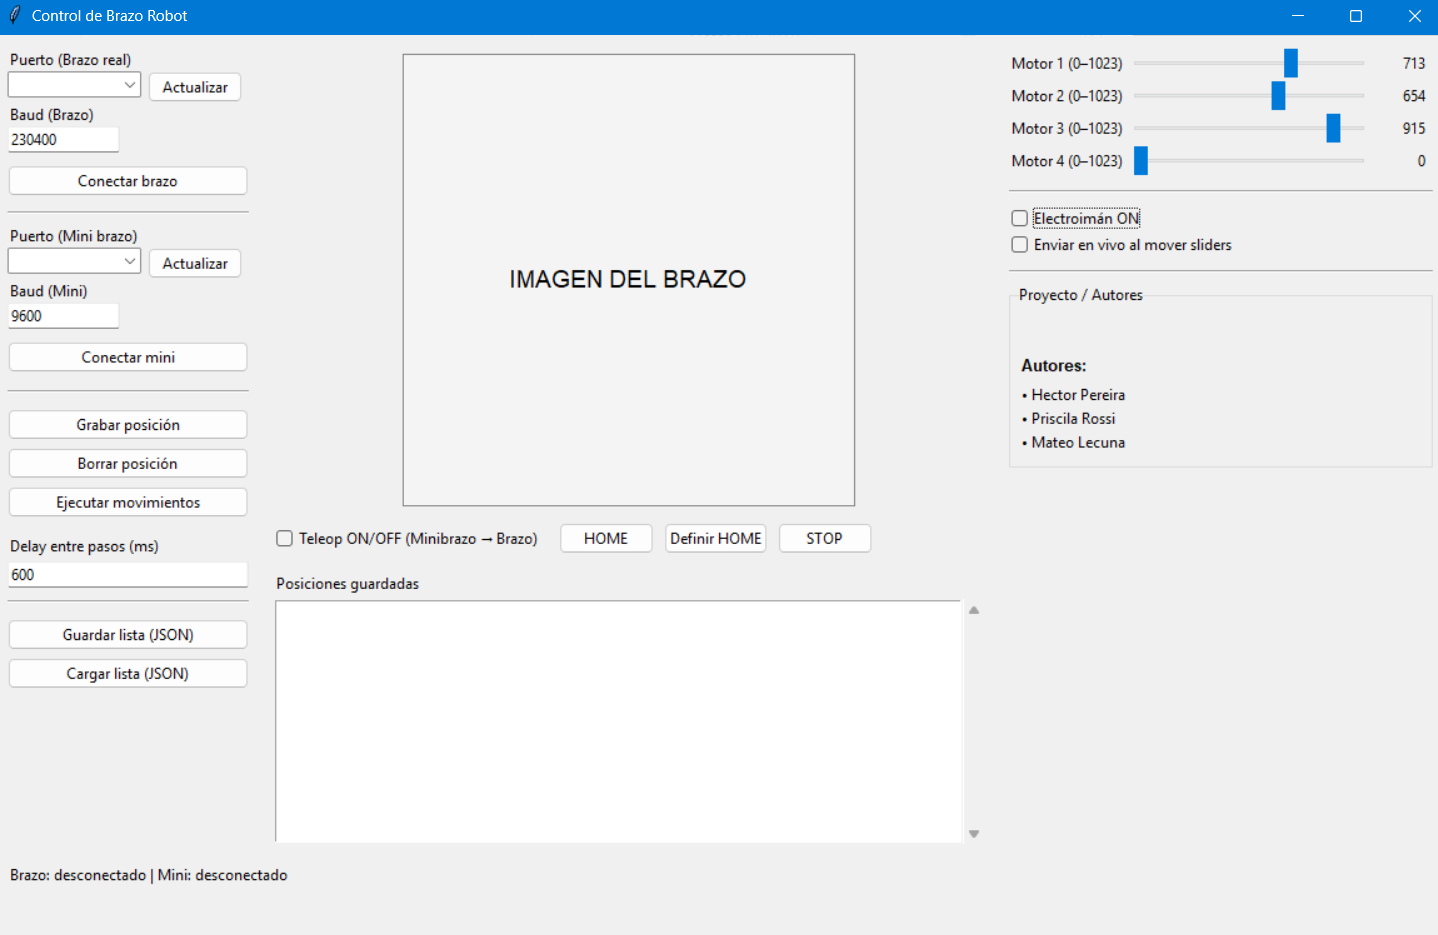
\includegraphics[width=0.8\textwidth]{anexos/software/ventanaApp.png}
  \caption{Captura de pantalla de aplicación (Fuente: elaboración própia)}\label{fig:captura.ventanaApp}
\end{figure}

Con el fin de complementar el diseño y la construcción del brazo robótico, se desarrolló una aplicación en Python que permite controlar el sistema de manera sencilla e intuitiva. El objetivo principal de esta aplicación es poder manejar el brazo desde la PC, ya sea mediante una conexión por cable o USB o por medio de un módulo bluetooth.

Dentro de las funciones más importantes de la aplicación se destaca la posibilidad de utilizar mini brazo como mando. Este dispositivo cuenta con potenciometros en sus articulaciones, lo que permite manipular los parametros de la aplicación en tiempo real. De esta manera, al mover el mini brazo se reflejan los cambios directamente en el brazo real, logrando un control simultáneo y fácil de comprender.

Otra de las características relevantes de la aplicación es el manejo de movimientos preguardados. El usuario puede realizar una secuencia de acciones paso a paso, ir guardando las posiciónes intermedias, y posteriormente reproducir ese movimientos de forma automática mediante la opción de "ejecutar movimientos". Además, la aplicación permite guardar estas secuencias en un archivo .json, y cargarlo nuevamente cuando sea necesario, lo cual facilita repetir rutinas sin necesidad de programar el brazo cada vez.

En cuanto a la interfaz, la aplicación se organizó de manera clara en 3 columnas principales. En el panel de la izquierda se encuentran las opciones de conexión con los brazos, la selección de puertos de comunicación y la configuración de la velocidad de transmisión de datos. El panel central muestra la representación del brazo junto con controles básicos de operación, y finalmente, en el panel de la derecha se ubican los sliders para ajustar manualmente cada articulación, además del control del electroimán. Esta distribución busca que el usuario pueda identificar fácilmente las funciones disponibles y operar el brazo de manera cómoda.

En resumen, la aplicación representa un avance importante dentro del proyecto, ya que no solo permite el control directo del brazo en tiempo real, sino que también posibilita la incorporación de un modelo físico de referencia (minibrazo) y la ejecución de secuencias guardadas, otorgando flexibilidad y versatilidad al sistema.
